\documentclass[12pt]{article}
% Эта строка — комментарий, она не будет показана в выходном файле
\usepackage{ucs}
\usepackage[warn]{mathtext} 
\usepackage[utf8x]{inputenc} % Включаем поддержку UTF8
\usepackage[russian]{babel}  % Включаем пакет для поддержки русского языка
\usepackage{amsmath}
\usepackage{mathtools}
\usepackage{amssymb}
% \usepackage[dvips]{graphicx}
% \graphicspath{{noiseimages/}}
\usepackage[pdftex]{graphicx}

\hoffset=0mm
\voffset=0mm
\textwidth=180mm        % ширина текста
\oddsidemargin=-6.5mm   % левое поле 25.4 - 5.4 = 20 мм
\textheight=240mm       % высота текста 297 (A4) - 40
\topmargin=-15.4mm      % верхнее поле (10мм)
\headheight=5mm      % место для колонтитула
\headsep=5mm          % отступ после колонтитула
\footskip=8mm         % отступ до нижнего колонтитула


\begin{document}
	\author {Жарков Андрей 496}
	\title {Лабораторная работа 1.5 \\ Изучение колебаний струны}
	\maketitle{}
	
	\indent
	\textbf{Цель работы:} изучение поперечных стоячих волн в струне: определение собственных частот колебания струны в зависимости от натяжения струны и определение скорости распространения поперечных волн в струне. 
	\\\newline
	\indent
	\textbf{В работе используются:} звуковой генератор, двухканальный осциллограф, частотомер, набор грузов, станина, с закрепленной на ней струной.
	
	\begin{center}
		\textbf{Теоретическое введение}
	\end{center}
	Ограниченная, закрепленная на концах струна, может совершать собственные колебания, представляющие собой стоячие волны вида
	$$y(x, t) = Asin(2\pi ft)sin(\frac{2\pi}{\lambda}x),$$
	где $A$ — амплитуда колебаний в пучностях, $f$ — частота, $\lambda$ — длина
	волны, $x$ — координата вдоль струны. В концевых точках должны располагаться узлы стоячей волны (амплитуда колебаний равна нулю), откуда
	следует, что на струне длиной L должно укладываться целое число полуволн:
	$$L = n\frac{\lambda_n}{2}, \ \ \ \ \ n = 1, 2, 3,...$$
	Скорость распространения поперечных волн $u$ зависит от силы натяжения струны $F$ и массы струны на единицу длины $\rho_l$ (погонной плотности
	струны $\rho_l = \rho S$): 
	\begin{equation}
	u = \sqrt{\frac{F}{\rho_l}}
	\end{equation} 
	Возможные частоты собственных колебаний струны (обертоны):
	\begin{equation}
	f_n = \frac{u}{\lambda_n} = \frac{n}{2L}\sqrt{\frac{F}{\rho_l}}
	\end{equation}
	Если частота внешней поперечной синусоидальной силы совпадает с
	какой либо собственной частотой колебания струны, то возникает явление
	резонанса и образуется синусоидальная стоячая волна.
	
	\begin{center}
		\textbf{Экспериментальная установка}
	\end{center}
	Схема установки показана на рисунке. Металлическая гитарная струна
	(1) закреплена в горизонтальном положении между двумя стойками (2)
	и (3), расположенными на массивной станине (4). Натяжение в струне создают грузы (5), подвешенные к концу струны, перекинутому через блок.
	Возбуждение и регистрация колебаний струны осуществляются с помощью электромагнитных катушек (датчиков), расположенных на станине
	под струной. На датчик (6), возбуждающий колебания струны в вертикальной плоскости, подаётся переменный синусоидальный сигнал от звукового генератора (7). Колеблющаяся струна возбуждает сигнал в регистрирующей катушке (8), который можно наблюдать на экране двухканального осциллографа (9). Датчики можно перемещать по станине. Разъёмы, соединяющие датчики с генератором и осциллографом, расположены
	на корпусе станины. Датчики следует повернуть так, чтобы магниты катушек были расположены перпендикулярно струне. Возбуждающий датчик
	следует расположить вблизи неподвижного конца струны, а регистрирующий — в максимуме отклонения струны от положения равновесия (пучности).
	\begin{center}
		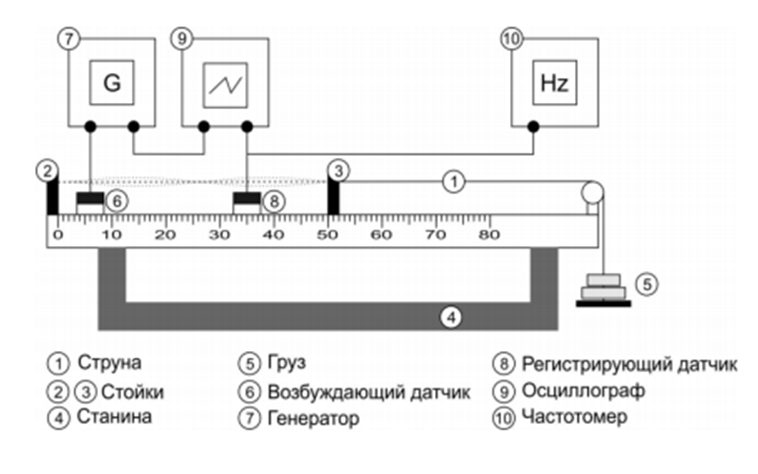
\includegraphics[width=4in]{5_1.png}
	\end{center}
	
	\begin{center}
		\textbf{Выполнение работы}
	\end{center}
	Параметры оборудования:\\
	$L$ = 80,0 см - длина струны \\
	$m_0$ = 58,0 г - масса платформы, крючков и кольца \\
	$m_1$ = 491,8 г, $m_2$ = 498,9 г, $m_3$ = 459,4 г, $m_4$ = 479,0 г, $m_5$ = 492,6 г - массы грузиков\\
	При различной общей массе подвешеных грузиков получились следующие результаты:\\
	\begin{center}
		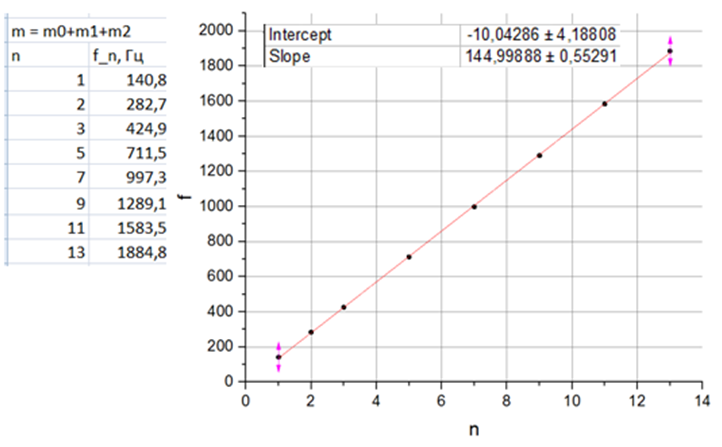
\includegraphics[width=4in]{5_2.png}\\
		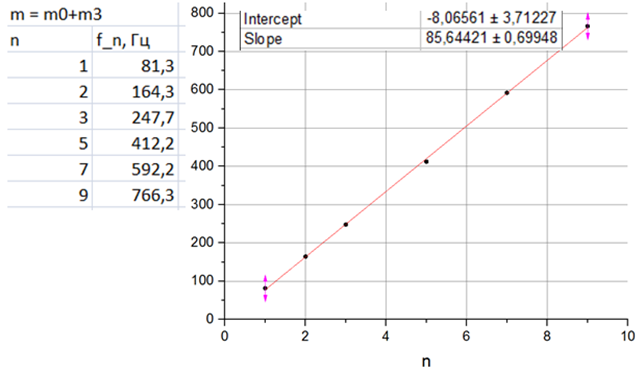
\includegraphics[width=4in]{5_3.png}\\
		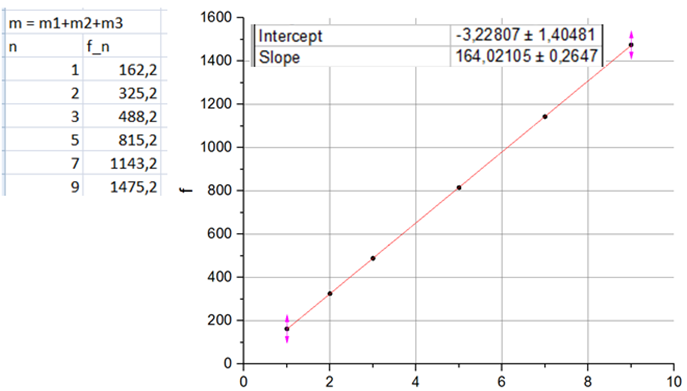
\includegraphics[width=4in]{5_4.png}\\
		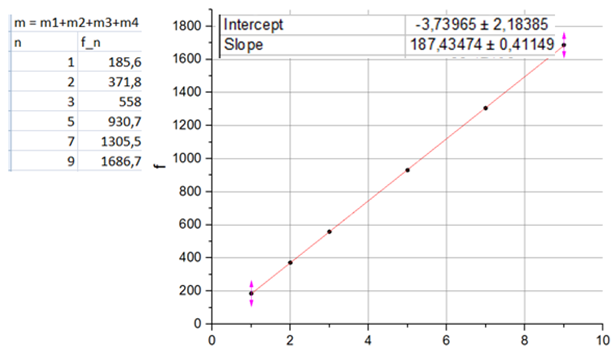
\includegraphics[width=4in]{5_5.png}\\
		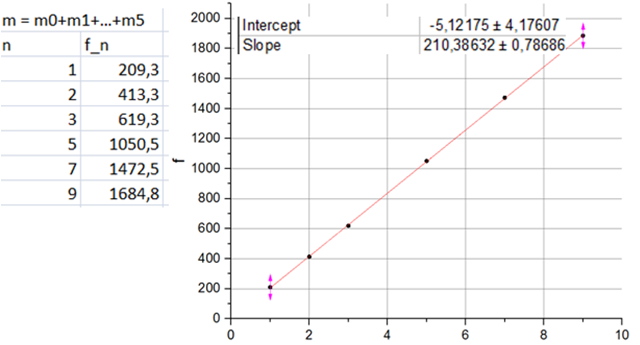
\includegraphics[width=4in]{5_6.png}\\
	\end{center}
	Из формулы (2) $f_n = kn$, $k = \frac{u}{2L}$, откуда $u = 2kL$ 
	\begin{center}
		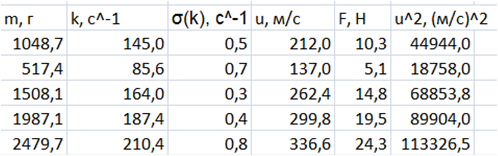
\includegraphics[width=4in]{5_7.png}\\
		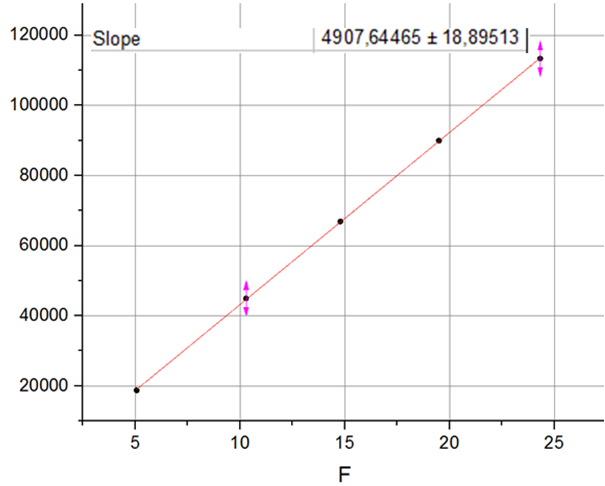
\includegraphics[width=4in]{5_8.png}\\
	\end{center}
	Из формулы (1) $u^2 = kF$, $k = \frac{1}{\rho_l}$, откуда $\rho_l = \frac{1}{k} = (2.04 \pm 0.03) * 10^{-4}$ $\frac{кг}{м}$, что в пределах погрешности равняется истинной погонной плотности установки ($\rho_l = 2.05 * 10^{-4}$ $\frac{кг}{м}$)

\end{document}